\section{Weronika Hilaszek}
\label{sec:whilaszek}
\vspace{0.4cm}

Here is a photo of the most beautiful bird (see Figure~\ref{fig:ptaszek}).

\begin{figure}[htbp]
    \centering
    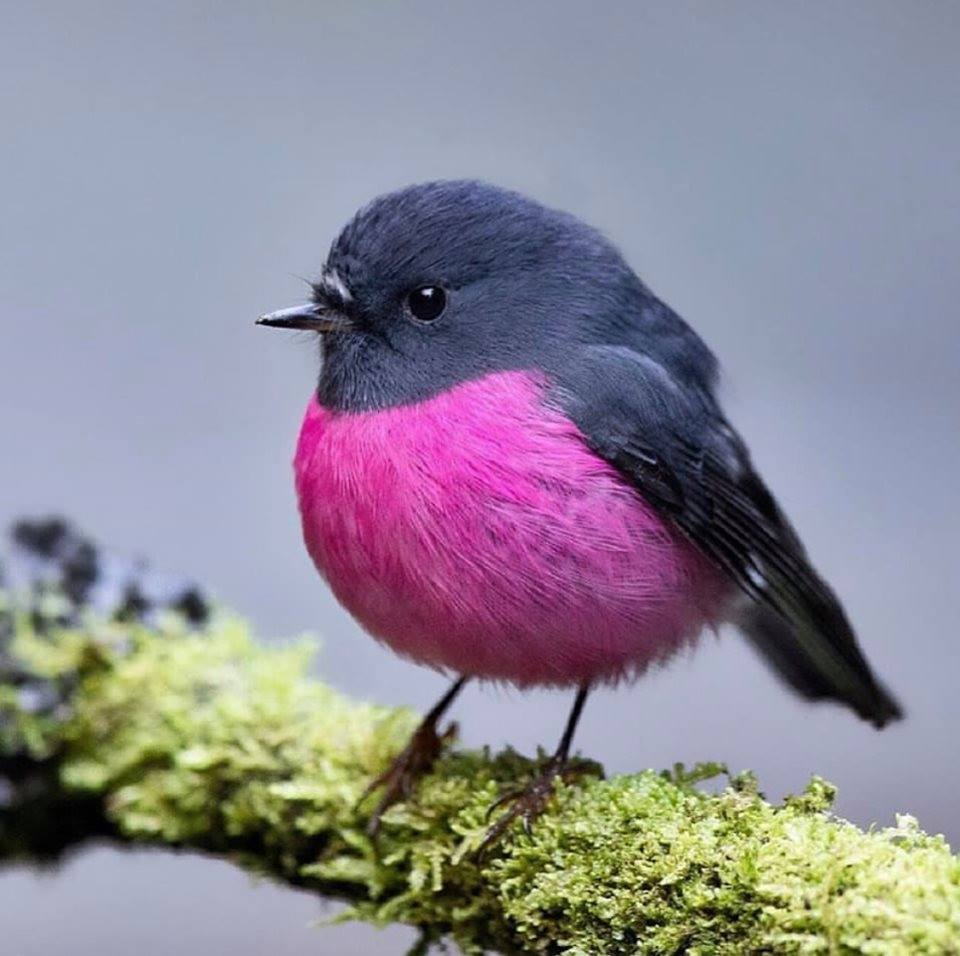
\includegraphics[width=0.5\textwidth]{Pictures/4_WHilaszek.jpg}
    \caption{This bird is a rose robin.}
    \label{fig:ptaszek}
\end{figure}
\vspace{1.0cm}

Table~\ref{tab:ptaszki} represents the life expectancy and flight speed of some birds.

\begin{table}[htbp]
\centering
\begin{tabular}{||c|c|c||}
 \hline
 Ptak & szybkość lotu & długość życia \\ [0.5ex]
 \hline\hline
 Jerzyk & 200km/h & 20 lat \\
 \hline
 Wróbel & 42km/h & 3 lata \\
 \hline
 Gołąb & 60km/h & 6 lat \\
 \hline
 Sroka & 30km/h & 12 lat \\
 \hline
 Kaczka & 65km/h & 5-10 lat \\
 \hline
\end{tabular}
\label{tab:ptaszki}
\caption{That is my table.}
\end{table}
\vspace{0.8cm}

Here is my equation: \[\sqrt{x^2+5}=25\]

And here is my function: $ f(x) = \frac{5}{x} $
\vspace{3.8cm}

My favorite birds:
\begin{enumerate}
    \item Blue tit
    \item Kestrel
    \item Bullfinch
    \item Long-tailed tit
    \item Kinglet
\end{enumerate}

\vspace{0.8cm}

And here are some birds that I don't like:
\begin{itemize}
\renewcommand{\labelitemi}{$-$}
    \item Magpie
    \item Cuckoo
    \item Jaybird
\end{itemize}

\vspace{0.8cm}

\setlength{\parindent}{10ex}
 {\textbf{The cuckoos} are generally medium-sized slender birds. Most species live in trees, though a sizeable minority are ground-dwelling. The family has a cosmopolitan distribution; the majority of species are tropical. Some species are migratory. The cuckoos feed on \underline{insects, insect larvae} and a variety of other animals, as well as fruit. Some species are \textbf{brood parasites, laying their eggs in the nests of other species and giving rise to the metaphor cuckoo's egg}, but the majority of species raise their own young.} \par
 
\setlength{\parindent}{10ex}
 {\emph{Cuckoos have played a role in human culture for thousands of years}, appearing in Greek mythology as sacred to the goddess Hera. In Europe, the cuckoo is associated with spring, and with cuckoldry, for example in Shakespeare's Love's Labour's Lost.\textbf{ In India, cuckoos are sacred to Kamadeva}, the god of desire and longing, whereas in Japan, the cuckoo symbolises \textbf{unrequited} \underline{love}.} \par
 
 




